\documentclass[10pt,a4paper]{article}

\usepackage{fontspec}
\usepackage[spanish,provide=*]{babel}
\usepackage[margin=1.9cm,top=1.7cm,bottom=1.7cm]{geometry}
\usepackage{graphicx}
\usepackage{booktabs}
\usepackage{caption}
\usepackage{float}
\usepackage{microtype}

\captionsetup{font=small,labelfont=bf,skip=3pt}
\setlength{\parindent}{0pt}
\setlength{\parskip}{0.42em}
\setlength{\textfloatsep}{7pt}
\setlength{\intextsep}{6pt}
\renewcommand{\arraystretch}{0.98}
\makeatletter
\renewcommand\section{\@startsection{section}{1}{\z@}{0.7em}{0.3em}{\normalfont\large\bfseries}}
\makeatother
\newcommand{\tag}[1]{\texttt{#1}}

\begin{document}

{\Large\bfseries Reconocimiento de entidades nombradas en español con BETO}\\[2pt]
{\small Andrés Felipe Pereira Ávila \quad·\quad Implementación: \texttt{ner\_conll2002.ipynb}}

\textbf{Resumen.} Se comparó BETO con el encoder congelado (modelo A) y con \textit{fine-tuning} completo (modelo B) en la partición española de CoNLL-2002. En prueba, B alcanza un F1 micro de \textbf{0.8678}, por encima del 0.80 exigido, frente a 0.7946 de A, con 1.51 veces su tiempo de entrenamiento.

\section{Preparación y exploración del corpus}

Se reconstruyeron las oraciones de \texttt{esp.train} (entrenamiento), \texttt{esp.testa} (validación) y \texttt{esp.testb} (prueba). En todas las oraciones palabras y etiquetas tienen la misma longitud. Cada partición contiene una secuencia que empieza con \tag{I-X}, inválida en IOB2; se convirtió en \tag{B-X}, igual que hace \texttt{conlleval}, para que esa entidad no se pierda de la referencia.

\begin{table}[H]
\centering\small
\caption{Tamaño de cada partición, entidades completas por tipo y longitud de las oraciones en palabras.}
\begin{tabular}{lrrrrrrrrrr}
\toprule
Partición & Oraciones & Palabras & Entidades & PER & ORG & LOC & MISC & Mediana & P99 & Máx. \\
\midrule
Entrenamiento & 8\,323 & 264\,715 & 18\,798 & 4\,321 & 7\,390 & 4\,914 & 2\,173 & 34 & 76 & 1\,238 \\
Validación & 1\,915 & 52\,923 & 4\,352 & 1\,222 & 1\,700 & 985 & 445 & 28 & 77 & 141 \\
Prueba & 1\,517 & 51\,533 & 3\,559 & 735 & 1\,400 & 1\,084 & 340 & 37 & 74 & 202 \\
\bottomrule
\end{tabular}
\end{table}

\begin{table}[H]
\centering\small
\caption{Distribución de etiquetas BIO (\% de las palabras de cada partición).}
\begin{tabular}{lrrrrrrrrr}
\toprule
Partición & \tag{O} & \tag{B-PER} & \tag{I-PER} & \tag{B-ORG} & \tag{I-ORG} & \tag{B-LOC} & \tag{I-LOC} & \tag{B-MISC} & \tag{I-MISC} \\
\midrule
Entrenamiento & 87.61 & 1.63 & 1.47 & 2.79 & 1.89 & 1.86 & 0.71 & 0.82 & 1.21 \\
Validación & 85.70 & 2.31 & 1.62 & 3.21 & 2.58 & 1.86 & 0.63 & 0.84 & 1.24 \\
Prueba & 88.01 & 1.43 & 1.23 & 2.72 & 2.14 & 2.10 & 0.63 & 0.66 & 1.08 \\
\bottomrule
\end{tabular}
\end{table}

\begin{figure}[H]
\centering
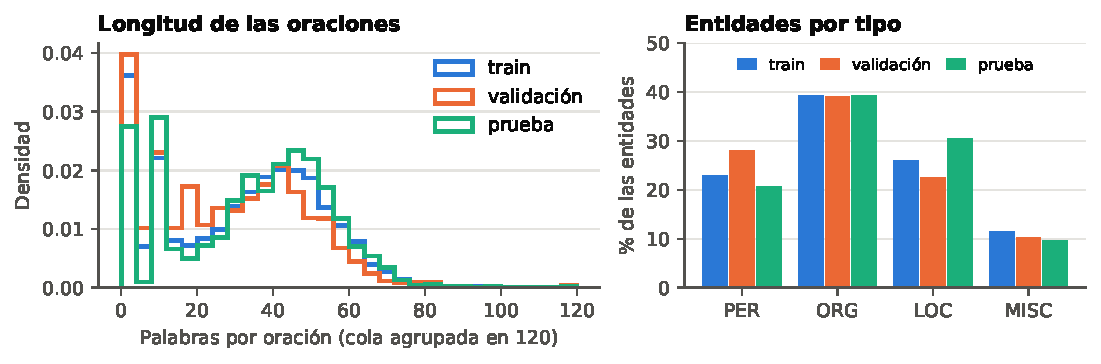
\includegraphics[width=0.74\linewidth]{figures/corpus.pdf}
\caption{Longitud de las oraciones y proporción de entidades por tipo en cada partición.}
\end{figure}

La clase \tag{O} domina: predecirla siempre daría una exactitud de 0.8801 en prueba, por lo que la métrica relevante es el F1 de entidades. \tag{ORG} es el tipo más frecuente; \tag{MISC}, el más escaso y el de entidades más largas (2.49 palabras de media). La longitud es bimodal, con muchos fragmentos de teletipo cortos, y su cola es extrema: una ``oración'' de 1\,238 palabras es un bloque sin segmentar. Prueba tiene más \tag{LOC} y menos \tag{PER} que validación. Ejemplos anotados de entrenamiento:

{\small
\begin{itemize}\setlength{\itemsep}{0pt}\setlength{\topsep}{0pt}\setlength{\parskip}{0pt}
\item \textbf{PER:} El alcalde , [José Luis Díez]\textsubscript{PER} , hablará sobre diversas cuestiones de interés municipal .
\item \textbf{ORG:} Como contrapartida , [Deutsche Telekom]\textsubscript{ORG} venderá al consorcio francés su participación del 25 por ciento en el empresa mixta británica [MetroHoldings]\textsubscript{ORG} .
\item \textbf{LOC:} 10:00 h. - [Jaraíz de la Vera]\textsubscript{LOC} ( [Cáceres]\textsubscript{LOC} ) .
\item \textbf{MISC:} Comenzará el Congreso \textquotedbl{} [Carlos. y el fin de una época. 1500-1558]\textsubscript{MISC} \textquotedbl{} .
\end{itemize}
}

\section{Alineación de etiquetas}

\textbf{Longitud máxima.} La decisión usó solo entrenamiento y validación. Se eligió \texttt{max\_length} = 384, el menor candidato que no afecta a ninguna entidad de validación. Con 128 subtokens se cubre el 99.7 \% de las oraciones, pero las truncadas son densas y validación perdería 62 entidades; con 256, 13. Con 384 solo se truncan 2 oraciones de entrenamiento (169 entidades afectadas) y ninguna de validación ni de prueba, cuya oración más larga tiene 289 subtokens. El costo es bajo porque el \textit{padding} es dinámico. El bloque más largo, de 3\,920 subtokens, debe truncarse en cualquier caso, ya que BERT admite 512 posiciones. Las métricas se calculan siempre contra la referencia completa.

\textbf{Alineación y verificación.} La función \texttt{align\_labels} recorre \texttt{word\_ids()}: etiqueta el primer subtoken de cada palabra y asigna \texttt{-100} a los tokens especiales y a los subtokens posteriores. El colador asigna \texttt{-100} al \textit{padding}. Una comprobación automática recorre todas las oraciones ya truncadas, con 384 y con un corte forzado a 32 subtokens: confirma el orden de las palabras, la etiqueta de cada primer subtoken y que ningún subtoken posterior quede etiquetado. Reconstruir las etiquetas por palabra recupera las 4\,352 entidades de validación y las 3\,559 de prueba.

\textbf{¿Por qué \texttt{-100}?} Es el \texttt{ignore\_index} de \texttt{CrossEntropyLoss}: esas posiciones no entran en la pérdida ni en su denominador y no generan gradiente. En los lotes de entrenamiento son el 62.6 \% de las posiciones (53.6 \% \textit{padding}, 6.7 \% subtokens posteriores, 2.4 \% especiales). Si se incluyeran como \tag{O}, los tokens sin etiqueta real aportarían ejemplos triviales: la pérdida bajaría sin mejorar el reconocimiento, el gradiente de las palabras reales se diluiría y la pérdida de una oración dependería de la longitud de sus vecinas de lote. Además, una palabra pesaría tanto como subtokens tenga, lo que sesgaría el ajuste hacia los nombres raros y fragmentados, en vez de optimizar la unidad que evalúa \texttt{seqeval}.

\begin{table}[H]
\centering\small
\caption{Palabras divididas en varios subtokens y sus etiquetas alineadas.}
\begin{tabular}{lll}
\toprule
Palabra & Subtokens & Etiquetas alineadas \\
\midrule
imposibilita & \texttt{imposi | \#\#bili | \#\#ta} & \tag{O | -100 | -100} \\
ZABALA & \texttt{Z | \#\#A | \#\#BA | \#\#LA} & \tag{B-PER | -100 | -100 | -100} \\
Commonwealth & \texttt{Common | \#\#w | \#\#eal | \#\#th} & \tag{B-ORG | -100 | -100 | -100} \\
Telekom & \texttt{Tele | \#\#k | \#\#om} & \tag{I-ORG | -100 | -100} \\
Cazoña & \texttt{Ca | \#\#zo | \#\#ña} & \tag{B-LOC | -100 | -100} \\
CrimeNet & \texttt{Cri | \#\#me | \#\#N | \#\#et} & \tag{B-MISC | -100 | -100 | -100} \\
\bottomrule
\end{tabular}
\end{table}

\section{Clasificación por token con BETO}

Ambos modelos se construyen con \texttt{AutoModelForTokenClassification} desde el mismo checkpoint, con la misma cabeza inicial, las 9 etiquetas, los mismos datos tokenizados (verificado con una huella) y la \texttt{CrossEntropyLoss} interna. Comparten también AdamW (\textit{weight decay} 0.01), calentamiento lineal del 10 \% y \textit{clipping} a 1.0. Se probaron LR $\in\{10^{-3},3\cdot10^{-3},10^{-2}\}$ en A y $\{2,3,5\}\cdot10^{-5}$ en B, con lotes de 16 y 32. La mejor época y la configuración se eligieron por F1 micro de validación, con parada temprana.

\begin{table}[H]
\centering\small
\caption{Configuración seleccionada para cada modelo.}
\setlength{\tabcolsep}{4.5pt}
\begin{tabular}{lrrrrrr}
\toprule
Modelo & LR & Lote & Parámetros entrenables & Épocas (mejor) & F1 val. búsqueda & Tiempo (min) \\
\midrule
A: encoder congelado & $3\cdot10^{-3}$ & 16 & 6\,921 & 15 (11) & 0.7728--0.7801 & 5.87 \\
B: \textit{fine-tuning} & $3\cdot10^{-5}$ & 32 & 109\,267\,209 & 6 (3) & 0.8633--0.8771 & 8.86 \\
\bottomrule
\end{tabular}
\end{table}

\begin{figure}[H]
\centering
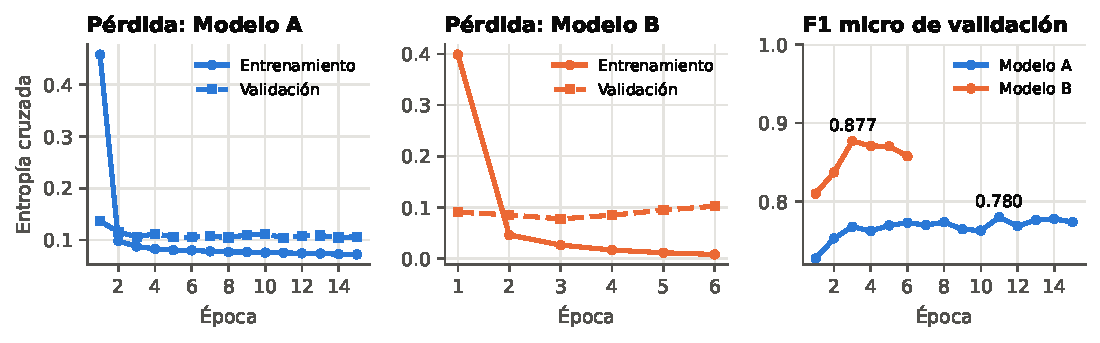
\includegraphics[width=0.86\linewidth]{figures/curvas.pdf}
\caption{Pérdida y F1 de validación de las configuraciones seleccionadas.}
\end{figure}

En A la pérdida de validación se estabiliza cerca de 0.106 desde la época 3 y no hay sobreajuste: el techo lo impone una capa lineal sobre representaciones fijas, y las seis configuraciones difieren menos de 0.008. En B la pérdida de validación toca su mínimo de 0.0776 en la época 3 y sube a 0.1025 en la época 6, mientras la de entrenamiento cae a 0.0082. Es sobreajuste claro, y por eso se conserva el estado de la época 3. El F1 varía alrededor de 0.01 entre épocas vecinas, así que la ventaja de 0.003 sobre la segunda mejor configuración no es concluyente.

\section{Evaluación final}

Cada modelo seleccionado se evaluó una sola vez sobre prueba; el resultado queda guardado y no se recalcula. Se usó \texttt{seqeval} en modo estricto IOB2: una entidad es correcta solo si coinciden sus límites y su tipo.

\begin{table}[H]
\centering\small
\caption{Métricas de entidades completas en prueba y exactitud por token sin \textit{padding} (51\,533 palabras).}
\begin{tabular}{lrrrrrrr}
\toprule
& \multicolumn{3}{c}{Modelo A} & \multicolumn{3}{c}{Modelo B} & \\
\cmidrule(lr){2-4}\cmidrule(lr){5-7}
& Precision & Recall & F1 & Precision & Recall & F1 & Soporte \\
\midrule
Micro global & 0.7931 & 0.7960 & 0.7946 & 0.8624 & 0.8733 & \textbf{0.8678} & 3\,559 \\
Macro entre tipos & 0.7570 & 0.7555 & 0.7556 & 0.8331 & 0.8543 & 0.8426 & 3\,559 \\
PER & 0.9195 & 0.9483 & 0.9337 & 0.9637 & 0.9755 & 0.9696 & 735 \\
ORG & 0.7589 & 0.8093 & 0.7833 & 0.8545 & 0.8807 & 0.8674 & 1\,400 \\
LOC & 0.8451 & 0.7703 & 0.8060 & 0.8917 & 0.8432 & 0.8668 & 1\,084 \\
MISC & 0.5045 & 0.4941 & 0.4993 & 0.6224 & 0.7176 & 0.6667 & 340 \\
\midrule
Exactitud por token & \multicolumn{3}{r}{0.9759} & \multicolumn{3}{r}{0.9851} & \\
\bottomrule
\end{tabular}
\end{table}

\begin{table}[H]
\centering\small
\caption{Comparación de desempeño y costo. Los errores son entidades de referencia no acertadas o predicciones espurias.}
\begin{tabular}{lrr@{\hspace{2.2em}}lrr}
\toprule
Medida & A & B & Errores en prueba & A & B \\
\midrule
F1 micro de validación & 0.7801 & 0.8771 & Correctas & 2\,833 & 3\,108 \\
F1 micro de prueba & 0.7946 & 0.8678 & Tipo incorrecto & 264 & 244 \\
Parámetros entrenables & 6\,921 & 109\,267\,209 & Límite incorrecto & 234 & 139 \\
Tiempo de entrenamiento (min) & 5.87 & 8.86 & Tipo y límite incorrectos & 67 & 36 \\
Tiempo por época (s) & 23.5 & 88.6 & Omitidas & 161 & 32 \\
Tiempo hasta la mejor época (min) & 4.31 & 4.43 & Espurias & 78 & 39 \\
\bottomrule
\end{tabular}
\end{table}

\begin{figure}[H]
\centering
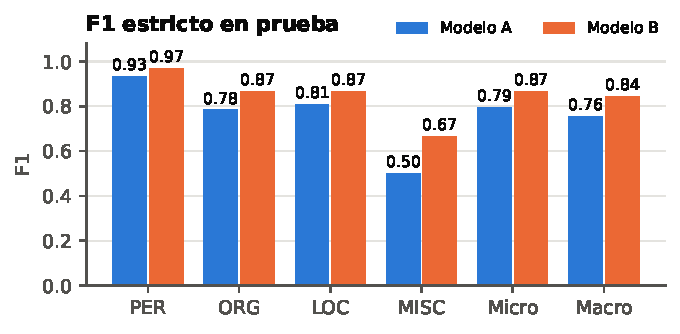
\includegraphics[width=0.46\linewidth]{figures/f1_por_entidad.pdf}\hfill
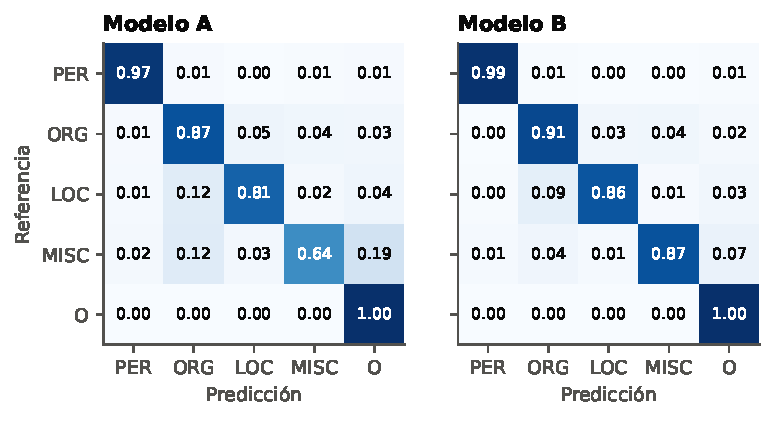
\includegraphics[width=0.50\linewidth]{figures/confusion.pdf}
\caption{F1 estricto en prueba (izquierda) y confusión por palabra entre tipos, normalizada por fila (derecha).}
\end{figure}

\textbf{Desempeño.} B gana en todas las métricas y cumple el requisito de 0.80. La mayor ganancia está en \tag{MISC} (+0.1674), que además explica que el F1 macro (+0.0870) mejore más que el micro (+0.0732). La exactitud por token solo sube 0.9 puntos porcentuales y oculta esa diferencia. Ajustar el encoder mejora sobre todo la detección y la delimitación: las omisiones bajan de 161 a 32 y los errores de límite de 234 a 139. Los errores de tipo casi no cambian y son 244 de los 451 fallos restantes de B, en buena parte por la confusión \tag{LOC}/\tag{ORG} (129 y 87 palabras), a menudo metonimia. Entre validación y prueba, A sube 0.0145 y B baja 0.0093; las particiones tienen distinta mezcla de tipos y parte del valor de validación de B puede ser optimismo de selección.

\textbf{Costo.} B entrena 15\,788 veces más parámetros y cada época tarda 3.77 veces más, pero se detiene antes, así que su tiempo total es solo 1.51 veces mayor y ambos llegan a su mejor época en unos 4.3--4.4 min. La búsqueda completa costó 63.4 min en B y 35.4 min en A. Esta última cifra está probablemente sobreestimada: algunas épocas de A tardaron hasta 45 s frente a los 23 s habituales, quizá por carga de la máquina, aunque la corrida seleccionada se mantuvo entre 23 y 25 s. A ejecuta el encoder en cada paso; cachear sus salidas lo abarataría mucho.

\textbf{Conclusión.} Conviene el \textit{fine-tuning}: aporta 0.0732 de F1 micro por un 51 \% más de tiempo. El modelo congelado solo se justifica con un presupuesto de cómputo muy limitado, y a costa de un \tag{MISC} con F1 de 0.4993.

\end{document}
